\documentclass{beamer}
\beamertemplatenavigationsymbolsempty
\usepackage{amsmath, amssymb, hyperref, graphics, tikz}
%\usepackage{mathpazo, soul}



\newcommand{\C}{\mathbb{C}}
\newcommand{\Z}{\mathbb{Z}}
\newcommand{\R}{\mathbb{R}}
\newcommand{\N}{\mathbb{N}}
\DeclareMathOperator{\Real}{Re}
\DeclareMathOperator{\Imag}{Im}


\begin{document}

\begin{frame}{Help prevent infections and disruptions from your studies}
\begin{itemize}
\item Wear masks inside if you can
\item Do not come onto campus if you have COVID-19 symptoms
\end{itemize}

\begin{block}{Last year's videos are available on Blackboard.}
\end{block}
\end{frame}

  \begin{frame}{Housekeeping: Office Hours}

Office hours mean I'm in my office for people to drop in and chat.  Take advantage of them!  I tried to pick office hours with few/no clashes with level 3 lectures, and set at half-hours to make it likely you can make part of them.

\begin{block}{Office Hours:}
\begin{itemize}
\item Wednesday 11:30-12:30 (online Blackboard Collaborate)
  \item Friday 14:30-15:30 (in my office, J06b)
\end{itemize}
\end{block}

These are subject to change; if you'd like to come a few times and those will never work, let me know, and maybe I'll change them!  You can also email to try to set up another time to drop in.

\end{frame}


\begin{frame}{Section 1.3: Inequalities}
Covered 1.1 Yesterday.  1.2 is worked examples!
\begin{lemma}[Triangle Inequality]For $z,w\in\C$ we have
\begin{eqnarray*}
\big| |z|-|w|\big| \leq |z+w| \leq |z|+|w| \\
\big| |z|-|w|\big| \leq |z-w| \leq |z|+|w| 
\end{eqnarray*}

\end{lemma}
 \begin{proof}
 The two inequalities are equivalent:  replace $w$ with $-w$.
 \begin{itemize}
     \item Consider the triangle with vertices $0, z$ and $z+w$.
     \item The sum of any two sides lengths is $\geq$ the third side length  
     \item Use this for all three sides and repackage 
\end{itemize}
 \end{proof}
  \end{frame}

\begin{frame}{Worked example of triangle inequality}


Show that for $z$ with $|z+2i|\leq 1$ we have
$$\frac{1}{\sqrt{5}+1}\leq \left|\frac{z}{z+1}\right| \leq \frac{3}{\sqrt{5}-1}$$  
 
\begin{block}{General Hints and ideas} 
 \begin{itemize}
     \item Treat denominator and numerator separately
     \item Rewrite what you want in terms of what you know
     \item Be careful of the direction of your inequalities
     \item Drawing a picture can help...
 \end{itemize}
 
 
 \end{block} 
  \end{frame}

\begin{frame}
  
\begin{center}

\Huge

\usebeamercolor[fg]{frametitle}
Clicker Session \\
Turning Point app or \\
ttpoll.eu 

\end{center}

\end{frame}


    \begin{frame}[plain]
        \begin{tikzpicture}[remember picture,overlay]
            \node[at=(current page.center)] {
                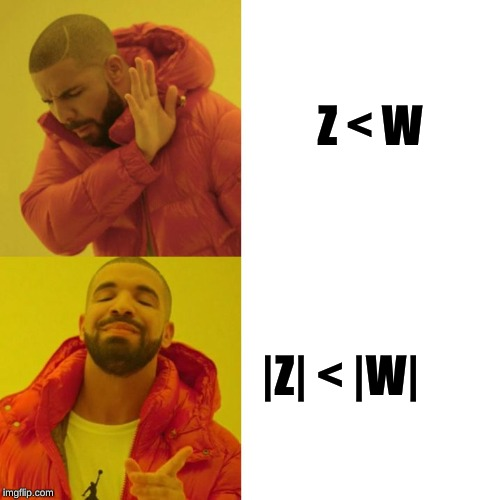
\includegraphics[keepaspectratio,
                                 width=\paperwidth,
                                 height=\paperheight]{DrakeInequality.jpg}
            };
        \end{tikzpicture}
     \end{frame}




\begin{frame}{Section 2: Special functions}

We won't sweat this, but defining $\exp(z)=e^z$ properly is tricky...  

\begin{definition}
$$\exp(x)=1+z+z^2/2+z^3/3!+\cdots=\sum_{n=0}^\infty \frac{z^n}{n!}$$
\end{definition}
Binomial theorem means $\exp(z)$ behaves like an exponential: $$\exp(z+w)=\exp(z)\exp(w)$$

And using Taylor series for $\sin(z)$ and $\cos(z)$ Euler's formula follows, and for $z=x+iy$
$$\exp(z)=e^x\left(\cos(y)+i\sin(y)\right)$$
So $\exp(z)$ is periodic with period $2\pi i$: $\exp(z+k2\pi i)=\exp(z)$.

\end{frame}

\begin{frame}{Other functions}
Using Euler's formula, for real $z$ we have
$$\cos(z)=\frac{e^{iz}+e^{-iz}}{2} \quad \quad \sin(z)=\frac{e^{iz}-e^{-iz}}{2i}$$
The right hand sides make sense for complex $z$, however, and so we can use these as the definition for $\sin(z)$ and $\cos(z)$ for $z\in\C$.
\begin{itemize}
    \item Still have $\cos^2(z)+\sin^2(z)=1$
    \item No longer have $|\sin(z)|\leq 1$!
\end{itemize}
\begin{block}{Hyperbolic versions: leave out the $i$}
$$\cosh(z)=\frac{e^{z}+e^{-z}}{2} \quad \quad \sinh(z)=\frac{e^{z}-e^{-z}}{2}$$
\end{block}
So $\sin(z)$ and $\cos(z)$ are periodic with period $2\pi$.
\end{frame}

\begin{frame}{Section 2.3 Worked examples}
\begin{block}{Example 1}
Find $M$ such that 
$$\left| \frac{e^z+\cos(z)}{z+6}\right| \leq M$$
for all $z$ with $|z|=1$.
\end{block}
\begin{block}{Example 2}
Find the zeroes of $\cos(z)$
\end{block}
\end{frame}
\end{document}
